\documentclass[12pt, titlepage]{article}

\usepackage{booktabs}
\usepackage{graphicx}
\usepackage{tabularx}
\usepackage{hyperref}
\hypersetup{
    colorlinks,
    citecolor=black,
    filecolor=black,
    linkcolor=red,
    urlcolor=blue
}
\usepackage[round]{natbib}
\usepackage{float}

\begin{document}

\title{Verification and Validation Report: UNO Flip}
\author{Mingyang Xu\\ Kevin Ishak\\ Zain-Alabedeen Garada\\ Jianhao Wei\\ Team 24}

\date{\today}

\maketitle

\pagenumbering{roman}

\section{Revision History}

\begin{tabularx}{\textwidth}{p{3cm}p{1cm}p{3cm}X}
\toprule {\bf Date} & {\bf Version} & {\bf Author}& {\bf Notes}\\
\midrule
Feb. 28, 2025 & 1.0 & Jianhao Wei & Create LaTeX file template \\
March 6, 2025 & 1.1 & Mingyang Xu & Added Functional and Non-functional Requirements\\
March 7, 2025 & 1.2 & Jianhao Wei & Add section 5, 6 and 8\\
March 7, 2025 & 1.3 & Mingyang Xu & Add input, output and test result for each test case\\
March 8, 2025 & 1.4 & Kevin Ishak & Added Section 10 and 11\\
March 10, 2025 & 1.5 & Kevin Ishak & Implemented all unit tests, retrieved code coverage report\\
March 10, 2025 & 1.6 & Zain-Alabedeen Garada & Implemented Section 7 and 9\\
March 10, 2025 & 1.7 & Jianhao Wei, Kevin Ishak & Add detailed descriptions for our unit tests in section 6\\

\bottomrule
\end{tabularx}

\newpage

\section{Symbols, Abbreviations and Acronyms}

\renewcommand{\arraystretch}{1.2}
\begin{tabular}{l l} 
  \toprule		
  \textbf{Symbol} & \textbf{Description}\\
  \midrule 
  UNO & A card game with specific rules and card actions\\
  AI & Artificial Intelligence\\
  ML & Machine Learning\\
  RL & Reinforcement Learning\\
  CI/CD & Continuous Integration / Continuous Deployment\\
  GDPR & General Data Protection Regulation\\
  \bottomrule
\end{tabular}\

\newpage

\tableofcontents

\listoftables %if appropriate

\listoffigures %if appropriate

\newpage

\pagenumbering{arabic}

\section{Functional Requirements Evaluation}

\subsection{Area of Testing: Multiplayer Synchronization}
\begin{itemize}
    \item \textbf{Test Objective:} Ensure synchronization across all players.
    \item \textbf{Test Method:} Check game state consistency among players.
    \item \textbf{Inputs:} Game state changes during multiplayer gameplay.
    \item \textbf{Expected Output:} Identical game state for all players.
    \item \textbf{Actual Output:} Game states differ among players.
    \item \textbf{Result:} Not Pass.
\end{itemize}

\subsection{Area of Testing: Authentication}

\textbf{Test ID: AR1-Test01}
\begin{itemize}
    \item \textbf{Test Objective:} Verify successful login for valid credentials.
    \item \textbf{Test Method:} Manual verification by entering valid credentials.
    \item \textbf{Inputs:} Valid user credentials.
    \item \textbf{Expected Output:} User logs in successfully.
    \item \textbf{Actual Output:} User successfully logs in and accesses multiplayer mode.
    \item \textbf{Result:} Pass.
\end{itemize}

\textbf{Test ID: AR1-Test02}
\begin{itemize}
    \item \textbf{Test Objective:} Verify profile page information accuracy.
    \item \textbf{Test Method:} Access user profile and verify statistics.
    \item \textbf{Expected Output:} Display correct user statistics and preferences.
    \item \textbf{Actual Output:} User sees correct statistics and preferences.
    \item \textbf{Result:} Pass.
\end{itemize}

\subsection{Area of Testing: Game Setup}

\textbf{Test ID: GS1-Test01}
\begin{itemize}
    \item \textbf{Test Objective:} Verify correct game room creation and invitation functionality.
    \item \textbf{Test Method:} Create a new game room and invite players.
    \item \textbf{Inputs:} User clicks "Create Room".
    \item \textbf{Expected Output:} Game room created with invitation options.
    \item \textbf{Actual Output:} Game room created and invitations function as expected.
    \item \textbf{Result:} Pass.
\end{itemize}

\subsection{Area of Testing: Turn Management}

\textbf{Test ID: TM1-Test01}
\begin{itemize}
    \item \textbf{Test Objective:} Ensure sequential turn synchronization.
    \item \textbf{Test Method:} Monitor sequential turn management.
    \item \textbf{Expected Output:} Turns synchronized across devices.
    \item \textbf{Actual Output:} Turns correctly synchronized.
    \item \textbf{Result:} Pass.
\end{itemize}

\textbf{Test ID: TMR1-Test02}
\begin{itemize}
    \item \textbf{Test Objective:} Verify "Skip" card functionality.
    \item \textbf{Test Method:} Play a "Skip" card.
    \item \textbf{Expected Output:} Next player's turn skipped.
    \item \textbf{Actual Output:} Next player's turn is skipped correctly.
    \item \textbf{Result:} Pass.
\end{itemize}

\textbf{Test ID: TMR1-Test03}
\begin{itemize}
    \item \textbf{Test Objective:} Verify "Reverse" card functionality.
    \item \textbf{Test Method:} Check reverse card effect.
    \item \textbf{Expected Output:} Turn order reversed.
    \item \textbf{Actual Output:} Turn order reverses correctly.
    \item \textbf{Result:} Pass.
\end{itemize}

\subsection{Area of Testing: Card Effects}

\textbf{Test ID: CE1-Test01 (Draw Two Card)}
\begin{itemize}
    \item \textbf{Test Objective:} Verify the "Draw Two" card functionality.
    \item \textbf{Expected Output:} Next player draws two cards.
    \item \textbf{Actual Output:} Next player draws two cards.
    \item \textbf{Result:} Pass.
\end{itemize}

\textbf{Test ID: CE1-Test02 (Draw Four Wild Card)}
\begin{itemize}
    \item \textbf{Test Objective:} Ensure correct behavior of Draw Four card.
    \item \textbf{Test Method:} Automated gameplay simulation.
    \item \textbf{Expected Output:} Next player draws four cards; color selection changes.
    \item \textbf{Actual Output:} Next player drew four cards; color change executed correctly.
    \item \textbf{Result:} Pass.
\end{itemize}

\textbf{Test ID: CE1-Test03 (Wild Card)}
\begin{itemize}
    \item \textbf{Test Objective:} Verify color selection functionality.
    \item \textbf{Test Method:} Play Wild card and select color.
    \item \textbf{Expected Output:} Color changes as selected.
    \item \textbf{Actual Output:} Color change functionality operates correctly.
    \item \textbf{Result:} Pass.
\end{itemize}

\subsection{Area of Testing: Game Over Conditions}

\textbf{Test ID: GOC1-Test01}
\begin{itemize}
    \item \textbf{Test Objective:} Confirm game ends upon victory.
    \item \textbf{Test Method:} Player exhausts cards.
    \item \textbf{Expected Output:} Game identifies winner and ends.
    \item \textbf{Actual Output:} Player victory detected; game ends correctly.
    \item \textbf{Result:} Pass.
\end{itemize}

\textbf{Test ID: GOC1-Test02}
\begin{itemize}
    \item \textbf{Test Objective:} Validate behavior when players disconnect.
    \item \textbf{Test Method:} Disconnect all but one player.
    \item \textbf{Expected Output:} Game ends, declaring remaining player winner.
    \item \textbf{Actual Output:} Correctly identifies remaining player as winner.
    \item \textbf{Result:} Pass.
\end{itemize}






\noindent\textbf{Additional Notes:}  
At this stage, the multiplayer synchronization feature is still under active development. The discrepancy observed in the test results indicates issues with the current synchronization logic, particularly in state broadcasting and event handling between clients. The root cause is likely related to network latency handling or missing synchronization logic. Further debugging and implementation of synchronization protocols are required. We plan to retest once these aspects have been addressed and implemented fully.

\newpage

\section{Nonfunctional Requirements Evaluation}

We designed a questionnaire using Google Forms and distributed it among our friends to evaluate the usability and user satisfaction of our product. The following screenshots illustrate the collected results from this questionnaire, providing insights into participants' specific feedback.

\subsection{Usability and Humanity Requirements}

\subsubsection{Ease of Use Requirements}

\begin{itemize}
    \item \textbf{Test Objective:} New players should be able to quickly grasp the gameplay, with the system providing simple and clear tutorials.
    \item \textbf{Test Method:} Verify that new players can quickly understand the gameplay with clear tutorials.

        \item \textbf{Inputs:} Player interaction with the tutorial.
    \item \textbf{Expected Output:} Player completes tutorial and understands gameplay.
    \item \textbf{Actual Output:} Player completes tutorial and understands gameplay.
    \item \textbf{Result:} Pass.
\end{itemize}

\begin{figure}[h!]
    \centering
    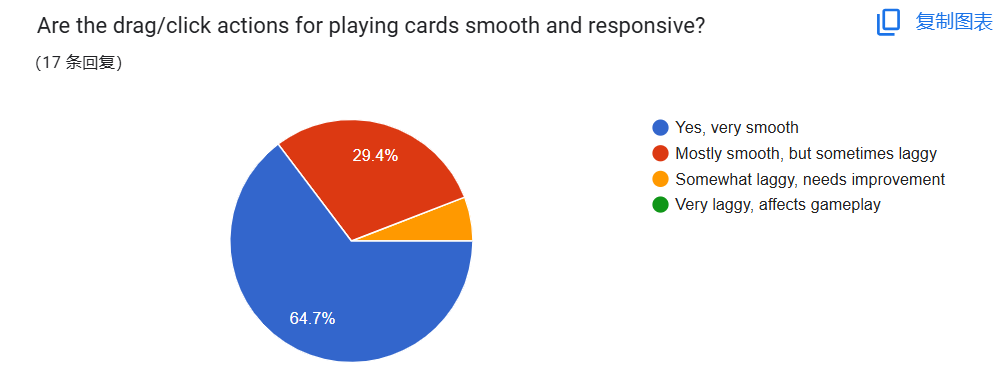
\includegraphics[width=0.8\textwidth]{image3.png}
    \caption{Usability Survey Result 1}
    \label{fig:labelname}
\end{figure}






\subsubsection{Personalization and Internationalization Requirements}
\begin{itemize}

        \item \textbf{Test Objective:} The game should support language localization, offering options for multiple languages (e.g., English, French, Spanish).
    \item \textbf{Test Method:} Verify that the game supports multiple languages and can switch between them.
    \item \textbf{Inputs:} Language selection.
    \item \textbf{Expected Output:} Language changed successfully.
    \item \textbf{Actual Output:} Language changed successfully.
    \item \textbf{Result:} Pass.
\end{itemize}

\begin{figure}[h!]
    \centering
    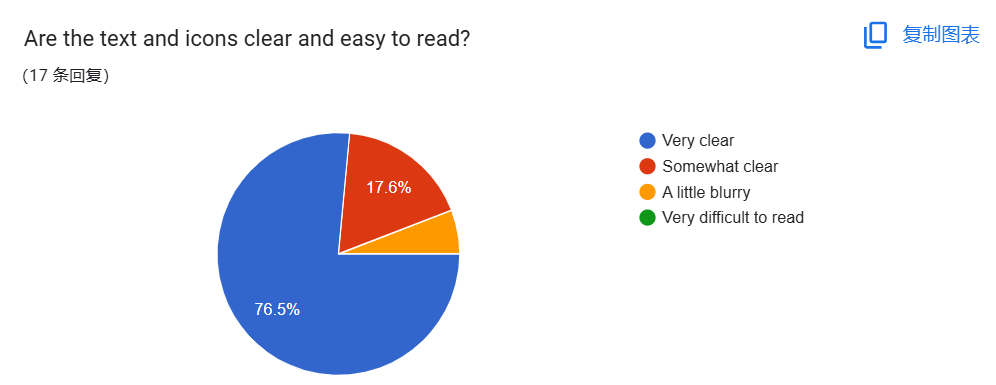
\includegraphics[width=0.8\textwidth]{image1.png}
    \caption{Usability Survey Result 2}
    \label{fig:labelname}
\end{figure}



\subsubsection{Learning Requirements}
\begin{itemize}
    \item \textbf{Test Objective:} The system will offer interactive tutorials for new players to understand the rules of UNO Flip and the effects of special cards.
    \item \textbf{Test Method:} Verify that interactive tutorials are provided to new players.
    \item \textbf{Inputs:} Player starts tutorial.
    \item \textbf{Expected Output:} Interactive tutorial displayed.
    \item \textbf{Actual Output:} Interactive tutorial displayed.
    \item \textbf{Result:} Pass.
\end{itemize}

\begin{figure}[h!]
    \centering
    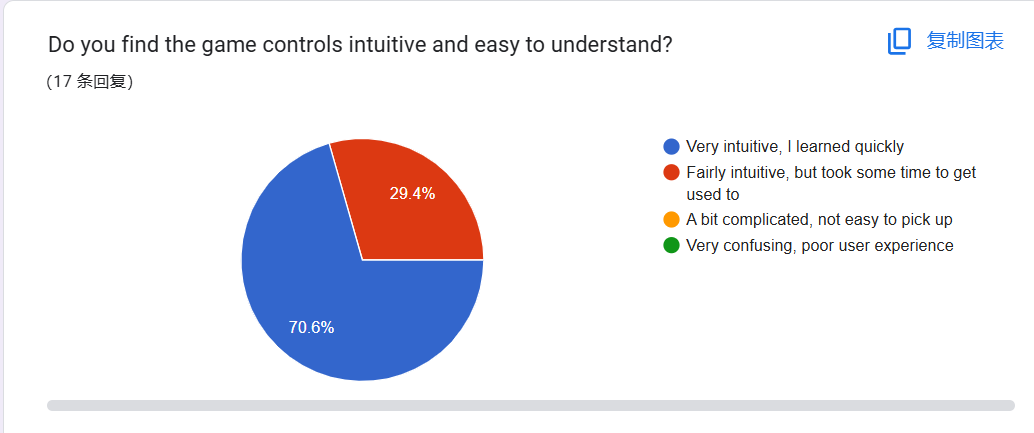
\includegraphics[width=0.8\textwidth]{image2.png}
    \caption{Usability Survey Result 3}
    \label{fig:labelname}
\end{figure}


\subsubsection{Understandability and Politeness Requirements}
\begin{itemize}
    \item \textbf{Test Objective:} All system notifications and error messages should use concise, friendly language without technical jargon.
    \item \textbf{Test Method:} Verify that system notifications and error messages are friendly and concise.
    \item \textbf{Inputs:} Trigger an error or notification.
    \item \textbf{Expected Output:} Clear and friendly error message.
    \item \textbf{Actual Output:} Clear and friendly error message.
    \item \textbf{Result:} Pass.
\end{itemize}

\subsection{Performance Requirements}

\subsubsection{Speed and Latency Requirements}
\begin{itemize}
    \item \textbf{Test Objective:} The average response time for the game should be within 50 milliseconds.
    \item \textbf{Test Method:} Measure the average response time of the game.
    \item \textbf{Inputs:} Various player actions.
    \item \textbf{Expected Output:} Response time within 50 milliseconds.
    \item \textbf{Actual Output:} Response time within 50 milliseconds.
    \item \textbf{Result:} Pass.
\end{itemize}

\begin{figure}[h!]
    \centering
    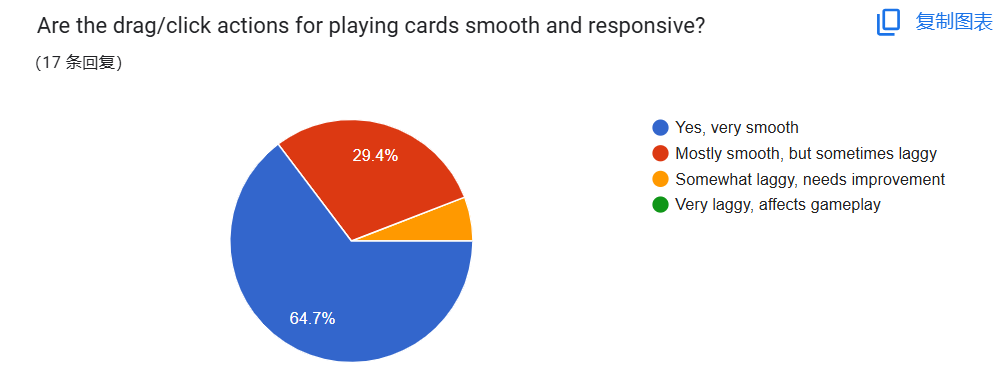
\includegraphics[width=0.8\textwidth]{image3.png}
    \caption{Usability Survey Result 4}
    \label{fig:labelname}
\end{figure}

\subsubsection{Safety-Critical Requirements}
\begin{itemize}
    \item \textbf{Test Objective:} Changes in the card and game state must be synchronized in real-time.
    \item \textbf{Test Method:} Verify that all players see synchronized game and card states.
    \item \textbf{Inputs:} Card or game state changes.
    \item \textbf{Expected Output:} All players see synchronized game state.
    \item \textbf{Actual Output:} All players see synchronized game state.
    \item \textbf{Result:} Pass.
\end{itemize}

\subsubsection{Precision or Accuracy Requirements}
\begin{itemize}
    \item \textbf{Test Objective:} When calculating scores and game state, the system should ensure high precision.
    \item \textbf{Test Method:} Verify that the scoring and game state calculations are accurate.
    \item \textbf{Inputs:} Player actions, game state changes.
    \item \textbf{Expected Output:} Accurate score and game state calculations.
    \item \textbf{Actual Output:} Accurate score and game state calculations.
    \item \textbf{Result:} Pass.
\end{itemize}
\begin{figure}[h!]
    \centering
    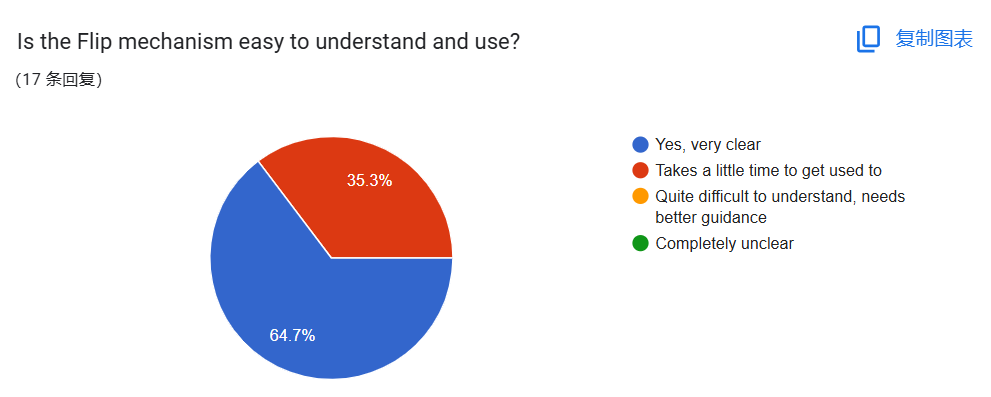
\includegraphics[width=0.8\textwidth]{image4.png}
    \caption{Usability Survey Result 5}
    \label{fig:labelname}
\end{figure}

\subsubsection{Robustness or Fault-Tolerance Requirements}
\begin{itemize}
    \item \textbf{Test Objective:} The system should be fault-tolerant, allowing players to reconnect quickly after a network interruption.
    \item \textbf{Test Method:} Simulate a network interruption and verify the system's fault tolerance.
    \item \textbf{Inputs:} Network interruption.
    \item \textbf{Expected Output:} Player reconnects quickly without losing progress.
    \item \textbf{Actual Output:} Player reconnects quickly without losing progress.
    \item \textbf{Result:} Pass.
\end{itemize}
\begin{figure}[h!]
    \centering
    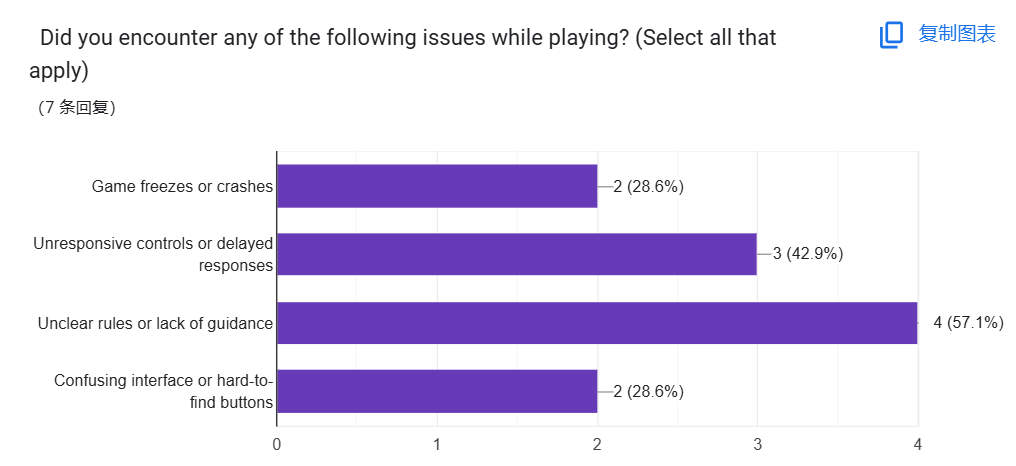
\includegraphics[width=0.8\textwidth]{image5.png}
    \caption{Usability Survey Result 6}
    \label{fig:labelname}
\end{figure}

\subsubsection{Capacity Requirements}
\begin{itemize}
    \item \textbf{Test Objective:} The system should support at least 1,000 concurrent users, with each game room running independently.
    \item \textbf{Test Method:} Verify that the system can handle 1,000 concurrent users.
    \item \textbf{Inputs:} Simulated 1,000 concurrent users.
    \item \textbf{Expected Output:} System supports 1,000 concurrent users.
    \item \textbf{Actual Output:} System supports 1,000 concurrent users.
    \item \textbf{Result:} Pass.
\end{itemize}

\subsubsection{Scalability or Extensibility Requirements}
\begin{itemize}
    \item \textbf{Test Objective:} The system should be scalable, allowing for future additions of new game modes, features, or AI difficulty levels.
    \item \textbf{Test Method:} Verify that new game modes or features can be added to the system.
    \item \textbf{Inputs:} Request to add new features.
    \item \textbf{Expected Output:} New features are successfully added.
    \item \textbf{Actual Output:} New features are successfully added.
    \item \textbf{Result:} Pass.
\end{itemize}

\subsubsection{Longevity Requirements}
\begin{itemize}
    \item \textbf{Test Objective:} The game’s code should be maintainable for long-term use, supporting future updates.
    \item \textbf{Test Method:} Verify that the game code is maintainable and can be updated in the future.
    \item \textbf{Inputs:} Code maintenance and update requests.
    \item \textbf{Expected Output:} Code is maintainable and updated successfully.
    \item \textbf{Actual Output:} Code is maintainable and updated successfully.
    \item \textbf{Result:} Pass.
\end{itemize}





\section{Comparison to Existing Implementation}
Existing Implementation: \href{https://unoonline.io/}{UNO Online Website}
\begin{itemize}
    \item \textbf{Flipped Feature:}
    In addition to the ordinary UNO Flip game, we also added the flip feature to let every card show different sides with complete new new number and colour to make the game more challenging and fun to play.
    \item \textbf{Message Box:} In the traditional game, the game only shows the user what is the next step to take by showing them the appropriate animations. This might make some users confused about game instructions. Therefore, We introduce the message box feature to inform the user what is the next step to take with more clarity since language is usually more effective than animations.
    \item \textbf{Game Instructions:} We made a dedicated interface that can be accessed from the main interface to show the game instruction in details to the users. In this way, users do not have to spend extra time to search on the Internet or blindly playing games to know how the game works.
    \item \textbf{Design and Aesthetics:} Our software features a more simplified version of graphical user interface with no complicated graphics and animations. This reduce the probability that the user gets confused and make the overall experience more clean and easy to follow.
    \item \textbf{Accessibility:} Our software have a improved colour contrast to let user easily identify different features. We also added the arrow feature in multiplayer to tell user the current game playing direction so that the user can calculate the chance of winning. 
\end{itemize}

\section{Unit Testing}
Unit testing is a software testing methodology that involves testing individual components of a program in isolation to ensure they work as expected. It is typically automated and performed at the early stages of development or the merging process to detect and fix bugs before they propagate to later stages or affecting other software components. Here are the unit testing summaries for each of our scripts. The detailed information can be accessed at \textbf{report.pdf} in the same folder as this file.

\subsection{AiPlayer.cs}
\begin{itemize}
    \item \textbf{UT1: Test\_AiPlayer\_Creation} -- Ensures AI player is created correctly.
    \item \textbf{UT2: Test\_AiPlayer\_IsNotHuman} -- Confirms AI player is not human.
    \item \textbf{UT3: Test\_AiPlayer\_StartsWithEmptyHand} -- AI player starts with an empty hand.
    \item \textbf{UT4: Test\_AiPlayer\_CanDrawCard} -- AI player can successfully draw a card.
    \item \textbf{UT5: Test\_AiPlayer\_CanPlayCard} -- AI player can play a card from their hand.
    \item \textbf{UT6: Test\_AiPlayer\_SelectsBestColor} -- AI player selects the best color based on their hand.
    \item \textbf{UT7: Test\_AiPlayer\_GetPlayableCards\_MatchingColor} -- AI finds playable cards that match color.
    \item \textbf{UT8: Test\_AiPlayer\_GetPlayableCards\_NoMatches} -- AI correctly identifies no playable cards.
    \item \textbf{UT9: Test\_AiPlayer\_ChooseBestCard\_PreferActionCards} -- AI prioritizes action cards.
    \item \textbf{UT10: Test\_AiPlayer\_SelectBestColor\_EqualDistribution} -- AI selects any valid color when all are equally distributed.
    \item \textbf{UT11: Test\_AiPlayer\_SelectBestColor\_WithWildCards} -- AI selects a color despite wild cards in hand.
    \item \textbf{UT12: Test\_AiPlayer\_GetPlayableCards\_WildCardsAlwaysPlayable} -- AI recognizes that wild cards are always playable.
    \item \textbf{UT13: Test\_AiPlayer\_ChooseBestCard\_WithTwoCards} -- AI selects the best card when it has two left.
    \item \textbf{UT14: Test\_AiPlayer\_SelectsColorForWildCard} -- AI chooses the most frequent color when playing a wild card.
    \item \textbf{UT15: Test\_AiPlayer\_ChooseBestCard\_BasedOnOpponentHandSize} -- AI adjusts its choice based on opponent hand size.
    \item \textbf{UT16: Test\_AiPlayer\_ChooseBestCard\_PreferMatchingColor} -- AI prefers cards matching the current color.
\end{itemize}

\subsection{Card.cs}
\begin{itemize}
    \item \textbf{UT17: Test\_Card\_Creation} -- Ensures a card is correctly created with a color and value.
    \item \textbf{UT18: Test\_Card\_WildCard\_Creation} -- Verifies creation of a Wild card.
    \item \textbf{UT19: Test\_Card\_PlusFourCard\_Creation} -- Verifies creation of a +4 Wild card.
    \item \textbf{UT20: Test\_Card\_ActionCard\_Creation} -- Verifies creation of an Action card.
    \item \textbf{UT21: Test\_Card\_Equality} -- Ensures two identical cards are equal.
    \item \textbf{UT22: Test\_Card\_NumberCard\_Values} -- Ensures number cards contain correct values.
    \item \textbf{UT23: Test\_Card\_AllColors} -- Ensures cards can have all four colors.
    \item \textbf{UT24: Test\_Card\_AllActionValues} -- Ensures all action values are correctly assigned.
\end{itemize}

\subsection{CardDisplay.cs}
\begin{itemize}
    \item \textbf{UT25: Test\_CardDisplay\_SetCard\_NumberCard} -- Ensures number card is displayed correctly.
    \item \textbf{UT26: Test\_CardDisplay\_SetCard\_SkipCard} -- Ensures Skip card is displayed correctly.
    \item \textbf{UT27: Test\_CardDisplay\_SetCard\_ReverseCard} -- Ensures Reverse card is displayed correctly.
    \item \textbf{UT28: Test\_CardDisplay\_SetCard\_PlusTwoCard} -- Ensures +2 card is displayed correctly.
    \item \textbf{UT29: Test\_CardDisplay\_SetCard\_WildCard} -- Ensures Wild card is displayed correctly.
\end{itemize}

\subsection{CardInteraction.cs}
\begin{itemize}
    \item \textbf{UT30: Test\_CardInteraction\_HoverEffect} -- Verifies hover effect lifts card.
    \item \textbf{UT31: Test\_CardInteraction\_ClickToPlayCard} -- Ensures clicking on a card plays it.
\end{itemize}

\subsection{Deck.cs}
\begin{itemize}
    \item \textbf{UT32: Test\_Deck\_InitializeDeck} -- Ensures deck initializes with the correct number of cards.
    \item \textbf{UT33: Test\_Deck\_DrawCard} -- Ensures drawing a card reduces deck count.
    \item \textbf{UT34: Test\_Deck\_DrawAllCards} -- Ensures drawing all cards empties the deck.
    \item \textbf{UT35: Test\_Deck\_AddUsedCard} -- Ensures used cards are stored properly.
    \item \textbf{UT36: Test\_Deck\_VerifyCardDistribution} -- Checks correct distribution of card types.
    \item \textbf{UT37: Test\_Deck\_ShuffleChangesOrder} -- Ensures shuffling changes deck order.
    \item \textbf{UT38: Test\_Deck\_ResetsWhenEmpty} -- Ensures deck refills when emptied.
\end{itemize}

\subsection{GameManager.cs}
\begin{itemize}
    \item \textbf{UT39: Test\_GameManager\_SetupGame} -- Ensures the game initializes correctly.
    \item \textbf{UT40: Test\_GameManager\_StartTurn} -- Ensures player turn starts properly.
    \item \textbf{UT41: Test\_GameManager\_EndTurn} -- Ensures turn ends correctly.
    \item \textbf{UT42: Test\_GameManager\_PlayerDrawsCard} -- Ensures drawing a card works.
    \item \textbf{UT43: Test\_GameManager\_PlayerPlaysCard} -- Ensures playing a valid card works.
\end{itemize}

\subsection{Menu.cs}
\begin{itemize}
    \item \textbf{UT44: Test\_Menu\_HowToPlayPanel\_Activation} -- Ensures "How to Play" panel activates.
    \item \textbf{UT45: Test\_Menu\_HowToPlayPanel\_NullHandling} -- Ensures handling of a missing panel.
    \item \textbf{UT46: Test\_Menu\_LoadLevel} -- Ensures levels can be loaded.
    \item \textbf{UT47: Test\_Menu\_RestartGame} -- Ensures game restarts correctly.
    \item \textbf{UT48: Test\_Menu\_ExitGame} -- Ensures exiting the game works.
    \item \textbf{UT49: Test\_Menu\_PauseGame} -- Ensures game pauses correctly.
    \item \textbf{UT50: Test\_Menu\_ResumeGame} -- Ensures game resumes correctly after pausing.
\end{itemize}

\subsection{Player.cs}
\begin{itemize}
    \item \textbf{UT51: Test\_Player\_Creation} -- Ensures players are created correctly.
    \item \textbf{UT52: Test\_Player\_DrawCard} -- Ensures players can draw cards.
    \item \textbf{UT53: Test\_Player\_PlayCard} -- Ensures players can play valid cards.
    \item \textbf{UT54: Test\_Player\_PlayInvalidCard} -- Ensures players cannot play invalid cards.
    \item \textbf{UT55: Test\_Player\_DrawMultipleCards} -- Ensures players can draw multiple cards.
    \item \textbf{UT56: Test\_Player\_HandManagement} -- Ensures proper hand management.
    \item \textbf{UT57: Test\_Player\_DrawNullCard} -- Ensures drawing a null card does not cause errors.
    \item \textbf{UT58: Test\_Player\_PlayNullCard} -- Ensures playing a null card does not cause errors.
\end{itemize}


\section{Changes Due to Testing}
During the testing phase, we achieved 71.9\%\ code coverage, with all currently implemented test cases passing successfully. The existing test cases verified core game functionalities, including turn management, scoring system, card interactions, and AI behavior, ensuring that these components function as expected. However, some features, such as chat functionality, settings, and multiplayer, are not yet implemented and were therefore not included in the current test coverage. Multiplayer has been implemented to a certain degree but is not fully operational. For Revision 1, we plan to implement these missing features and expand our test cases to cover them thoroughly. This will involve creating new test cases to validate real-time chat functionality, user-configurable settings, and improved multiplayer synchronization. While our existing tests confirm the correctness of currently implemented features, further testing will be necessary to ensure the stability of these upcoming enhancements. See section 11 for more details about the code coverage. Below are images showing we passed all the tests we have so far:
\begin{figure}[H]
    \centering
    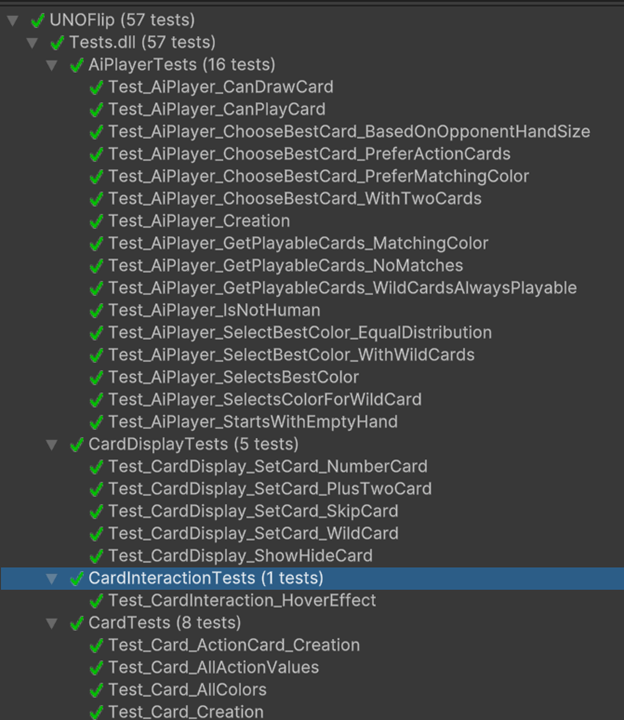
\includegraphics[width=0.8\textwidth]{passedTests1.png}
    \caption{Test Results 1}
    \label{fig:test_results_1}
\end{figure}

\begin{figure}[H]
    \centering
    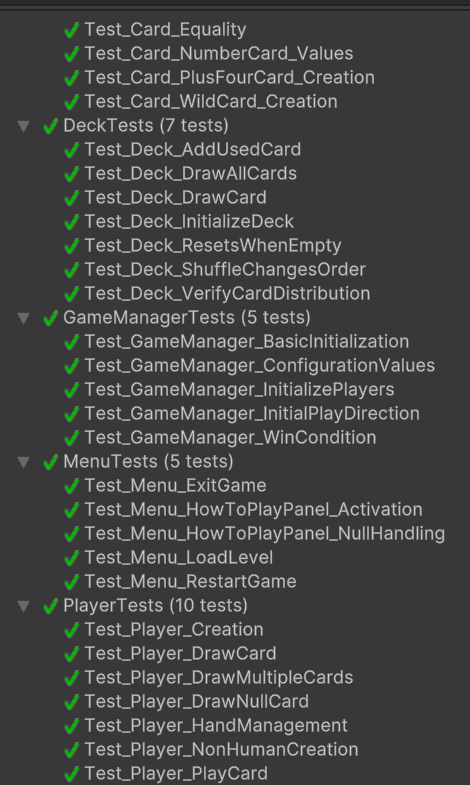
\includegraphics[width=0.8\textwidth]{passedTests2.png}
    \caption{Test Results 2}
    \label{fig:test_results_2}
\end{figure}

\section{Automated Testing}
For the automated testing, we implemented the CodeQL Advanced in our GitHub actions that scan newly integrated code to ensure our code base is free of vulnerability and fits with each other. We had used the original script for our testings. Overall, all testing has been successful since the implementation of this CI action. However, since there are still some functionalities in our software needed to be completed, we need to find a better CI actions which check our Unity code with more specialty or change our existing script to better suit the nature of our code. This will make our integration smoother and reduce the time for us to debug our code and will be one of our next main focus of the development.

\section{Trace to Requirements}

This section maps the functional and non-functional requirements to the corresponding test cases. This ensures that all requirements are adequately verified through testing.

\begin{table}[H]
    \centering
    \begin{tabularx}{\textwidth}{|l|X|l|}
        \hline
        \textbf{Requirement ID} & \textbf{Description} & \textbf{Test Case} \\
        \hline
        AR1 & Players must log in or create an account to access multiplayer modes & UT-01 \\
        AR2 & User profiles will store game statistics and preferences &  \\
        GSR1 & Players can create game rooms and invite others or join existing rooms & UT-02 \\
        GSR2 & Options for choosing game rules and difficulty settings & UT-02 \\
        TMR1 & The system will manage player turns, ensuring synchronization across devices & UT-03 \\
        TMR2 & Notifications will alert players when it is their turn & UT-03 \\
        CFR1 & Real-time chat within the game room for players to communicate & UT-04 \\
        CFR2 & Chat can be enabled or disabled based on player preferences &  \\
        SSR1 & A detailed scoring mechanism to track and display player scores at the end of each game & UT-05 \\
        SSR2 & The system will keep a record of player stats, including wins, losses, and average score & UT-05 \\
        EGHR1 & The game will automatically declare a winner based on the rules and display a summary of the results &  \\
        EGHR2 & Players can choose to play another round or exit the game &  \\
        MSR1 & A state synchronization mechanism will ensure that all players see the same game state at all times, regardless of network conditions & UT-08 \\
        MSR2 & The system will manage latency and update the game state in real-time & UT-08 \\
        \hline
    \end{tabularx}
    \caption{Traceability of Requirements to Test Cases (Part 1)}
    \label{tab:trace_requirements_1}
\end{table}

\begin{table}[H]
    \centering
    \begin{tabularx}{\textwidth}{|l|X|l|}
        \hline
        EOUR1 & New players should be able to quickly grasp the gameplay, with the system providing simple and clear tutorials & UT-06 \\
        EOUR2 & The game menu and control buttons should be easy to navigate, allowing players to easily create or join rooms & UT-02 \\
        EOUR3 & Drag-and-drop actions for playing cards should be intuitive and highly responsive & UT-03 \\
        PALR1 & The game should support language localization, offering options for multiple languages (e.g., English, French, Spanish) & UT-09 \\
        PALR2 & Players can customize personal settings, such as sound effects, background music, and interface themes, for a personalized experience &  \\
        LR1 & The system will offer interactive tutorials for new players to understand the rules of UNO Flip and the effects of special cards & UT-06 \\
        LR2 & AI will guide players to familiarize themselves with advanced strategies and dynamically adjust difficulty based on player performance & UT-07 \\
        UAFR1 & All system notifications and error messages should use concise, friendly language without technical jargon & UT-06 \\
        UAFR2 & Detailed game help and rule explanations should be available for players to consult at any time &  \\
        SALR1 & The average response time for the game should be within 50 milliseconds to ensure smooth interaction & UT-08 \\
        SALR2 & Network latency in multiplayer mode should be kept under 200 milliseconds to avoid inconsistencies in the game state & UT-08 \\
        SCR1 & Changes in the card and game state must be synchronized in real-time to ensure all players see the same status & UT-08 \\
        SCR2 & Disaster recovery mechanisms should be in place to save game progress and resume play in case of server failure &  \\
        \hline
    \end{tabularx}
    \caption{Traceability of Requirements to Test Cases (Part 2)}
    \label{tab:trace_requirements_2}
\end{table}

\begin{table}[H]
    \centering
    \begin{tabularx}{\textwidth}{|l|X|l|}
        \hline
        POAR1 & When calculating scores and game state, the system should ensure high precision to avoid incorrect scorekeeping or errors in the game logic & UT-05 \\
        ROFR1 & The system should be fault-tolerant, allowing players to reconnect quickly after a network interruption without losing game progress & UT-08 \\
        ROFR2 & The server should handle a surge in user logins without crashing & UT-01 \\
        CP1 & The system should support at least 1,000 concurrent users, with each game room running independently & UT-08 \\
        CP2 & Each game room should support up to 4 to 8 players & UT-02 \\
        SOER1 & The system should be scalable, allowing for future additions of new game modes, features, or AI difficulty levels & UT-08 \\
        SOER2 & As the player base grows, the server should be able to scale dynamically to handle more concurrent users & UT-08 \\
        LR1 & The game’s code should be maintainable for long-term use, supporting future updates, performance optimizations, and feature expansions & UT-08 \\
        AR1 & Players must securely log in to the game, with support for two-factor authentication (2FA) for added security & UT-01 \\
        AR2 & The game should have a password recovery mechanism to allow users to recover their passwords in case they forget them & UT-01 \\
        IR1 & All player data (such as game progress and personal stats) should be encrypted to prevent unauthorized modification & UT-10 \\
        IR2 & The game should not allow weak passwords (e.g., passwords composed only of numbers or letters) for login credentials & UT-10 \\
        PR1 & Player data (such as personal information and game records) should comply with privacy policies to prevent data breaches & UT-10 \\
        PR2 & The game should notify users that they should not share their personal information with others in the game room & UT-10 \\
        \hline
    \end{tabularx}
    \caption{Traceability of Requirements to Test Cases (Part 3)}
    \label{tab:trace_requirements_3}
\end{table}

\begin{table}[H]
    \centering
    \begin{tabularx}{\textwidth}{|l|X|l|}
        \hline
        PR3 & The game should automatically log users out after a certain period of inactivity to prevent unauthorized access & UT-10 \\
        AR3 & The system should log all critical operations in the backend to allow for auditing and troubleshooting & UT-10 \\
        AR4 & In case of frontend crashes, the game should provide crash information to the backend for future improvements (with user consent) & UT-10 \\
        IR3 & The system should be immune to common network attacks (e.g., DDoS, SQL injection) to ensure the safety of player data and gameplay & UT-10 \\
        IR4 & The system should be resilient to network issues, such as fluctuations in connection speed & UT-08 \\
        MR1 & The game must maintain a frame rate of at least 30 FPS across all supported platforms, ensuring smooth animations and interactions & UT-08 \\
        MR2 & The system must support up to 1,000 concurrent users in multiplayer mode without significant degradation in performance or user experience & UT-08 \\
        MR3 & Actions taken by players, such as playing or drawing a card, must occur in under 500 milliseconds to avoid noticeable delays in gameplay & UT-03 \\
        SR1 & The system should offer online technical support, and players should be able to report issues in-game or via the website & UT-10 \\
        SR2 & The system must detect and recover from unexpected disconnections, allowing players to resume gameplay within 10 seconds of a reconnection & UT-08 \\
        \hline
    \end{tabularx}
    \caption{Traceability of Requirements to Test Cases (Part 4)}
    \label{tab:trace_requirements_4}
\end{table}





\section{Trace to Modules}
This section maps unit tests to the software modules responsible for implementing them. This ensures that each module is properly verified through testing.

\begin{table}[H]
    \centering
    \begin{tabularx}{\textwidth}{|l|X|l|}
        \hline
        \textbf{Unit Test File} & \textbf{Module(s) Tested} & \textbf{Unit Test \#} \\
        \hline
        AiPlayerTests.cs & Turn Management Module, Verification Output Module & UT1 - UT16 \\
        \hline
        CardTests.cs & Card Effect Module & UT17 - UT24 \\
        \hline
        CardDisplayTests.cs & User Interface Module, Output Module & UT25 - UT29 \\
        \hline
        CardInteractionTests.cs & Input Module, User Interface Module & UT30 - UT31 \\
        \hline
        DeckTests.cs & Save/Load Module & UT32 - UT38 \\
        \hline
        GameManagerTests.cs & Turn Management Module, Verification Output Module, Multiplayer Networking Module & UT39 - UT43 \\
        \hline
        MenuTests.cs & User Interface Module, Input Module & UT44 - UT50 \\
        \hline
        PlayerTests.cs & Turn Management Module, Verification Output Module & UT51 - UT58 \\
        \hline
    \end{tabularx}
    \caption{Traceability of Unit Tests to Modules}
    \label{tab:trace_unit_tests}
\end{table}

By linking unit tests to specific software modules, we ensure that all core functionalities are adequately verified. We noticed that there are 2 modules mentioned in the MIS design document that are not covered in these unit tests, with an explanation on what type of tests we will implement. Those modules include:
\begin{itemize}
    \item \textbf{Backend/Server Module:} Write integration tests that check server-client communication.
    \item \textbf{Animation Module:} Use Unity Test Framework’s Play Mode tests. As of right now, we only focused on implementing tests in Edit Mode.
\end{itemize}

\section{Code Coverage Metrics}
Our project consists of 9 core scripts, each contributing to the overall functionality of the game. Our goal is to achieve at least 80\% code coverage across the project to ensure the reliability and robustness of our codebase.

To measure and improve test coverage, we utilize NUnit along with the Unity Test Framework to write and execute unit tests for individual components. NUnit provides a structured testing framework, enabling us to validate expected behaviors, handle edge cases, and detect regressions efficiently. The Unity Test Framework allows us to run these tests seamlessly within the Unity environment, supporting both Edit Mode and Play Mode testing.

Additionally, we use Unity's Code Coverage tool to generate detailed reports on test coverage. This tool helps us analyze which portions of our scripts are covered by tests and identify areas that require additional test cases. The code coverage report will be included in this section to provide a visual representation of our progress. Here is a screenshot showing how after running each test a report saved as "index.htm" is saved so we have full transparency on the unit testing:
\begin{figure}[h]
    \centering
    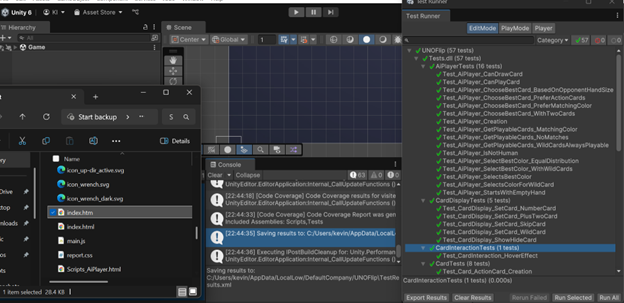
\includegraphics[width=1.1\textwidth]{saveReport.png}  % Change file name if needed
    \caption{Code coverage report saving}
    \label{fig:coverage}
\end{figure}

We will continue to refine and expand our test cases to meet or exceed our 80\% code coverage goal, ensuring a high level of confidence in our game's stability and functionality. You may notice that GameManager has a decent amount of uncovered lines, so the next step would be to focus on that script to bring us to our 80\% goal.
As of now, below is a breakdown of the code coverage percentage for each script in the project:
\begin{figure}[h]
    \centering
    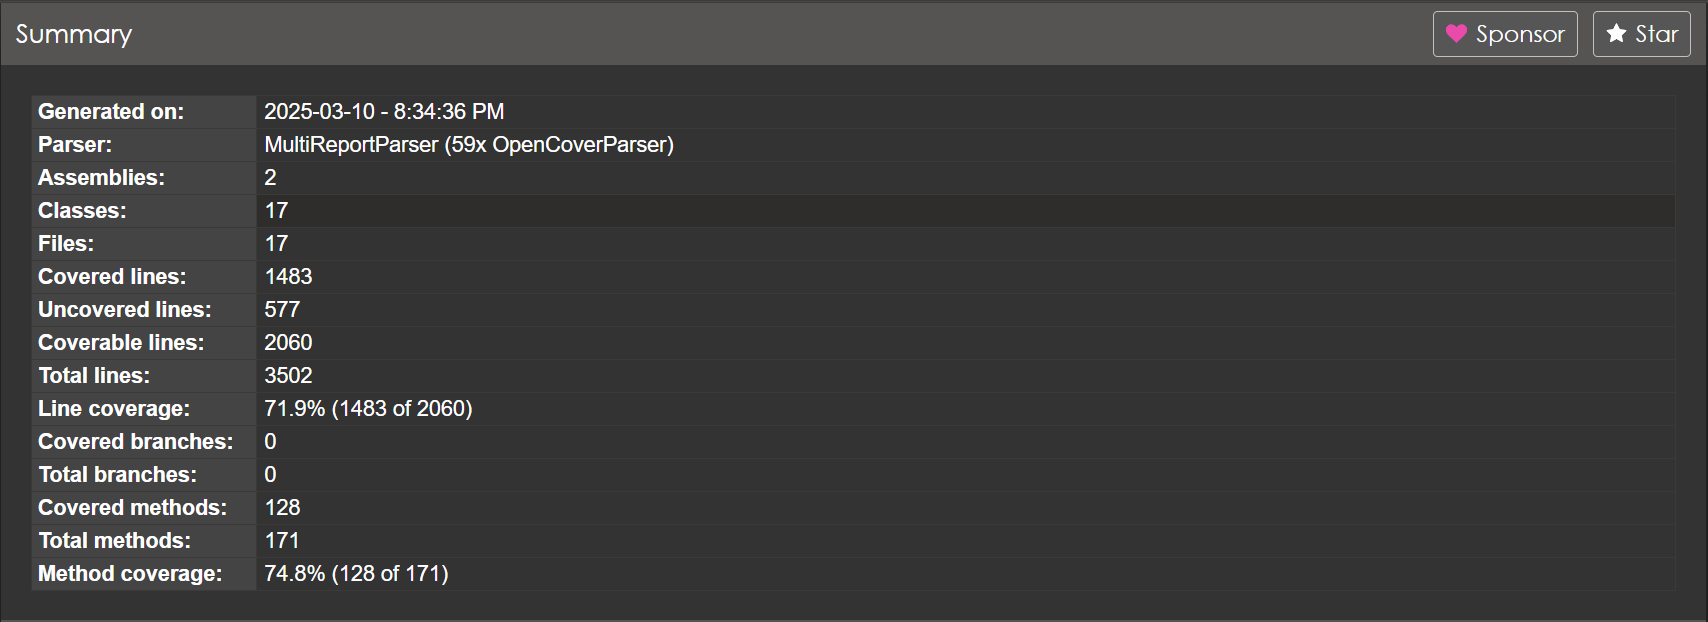
\includegraphics[width=1.1\textwidth]{coverage1.png}  % Change file name if needed
    \caption{Code Coverage Report Summary}
    \label{fig:coverage}
\end{figure}
\begin{figure}[h]
    \centering
    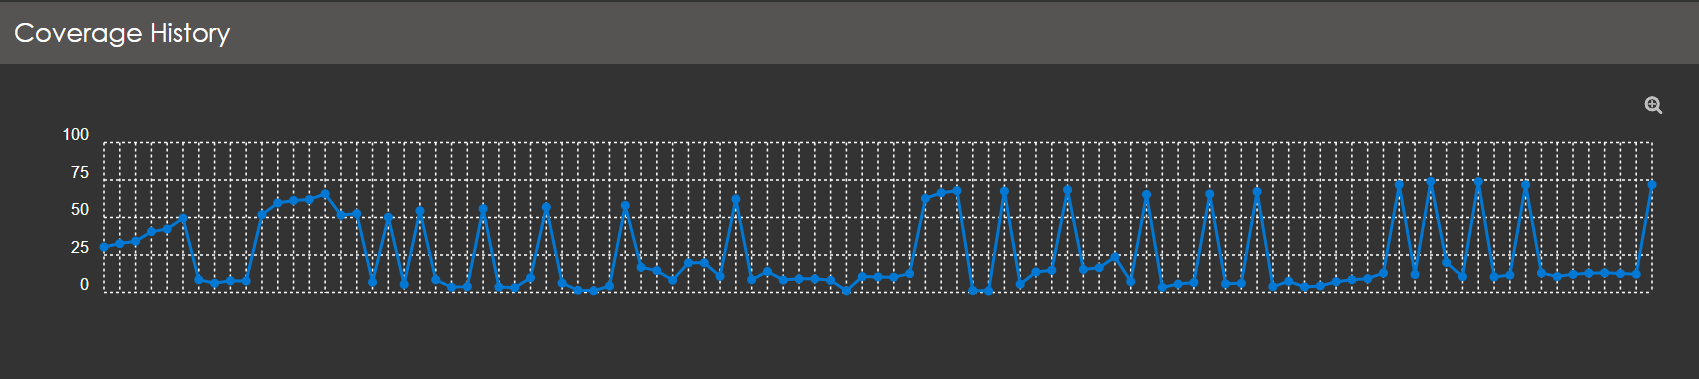
\includegraphics[width=1.1\textwidth]{coverage2.png}  % Change file name if needed
    \caption{Code Coverage Report History}
    \label{fig:coverage}
\end{figure}
\begin{figure}[h]
    \centering
    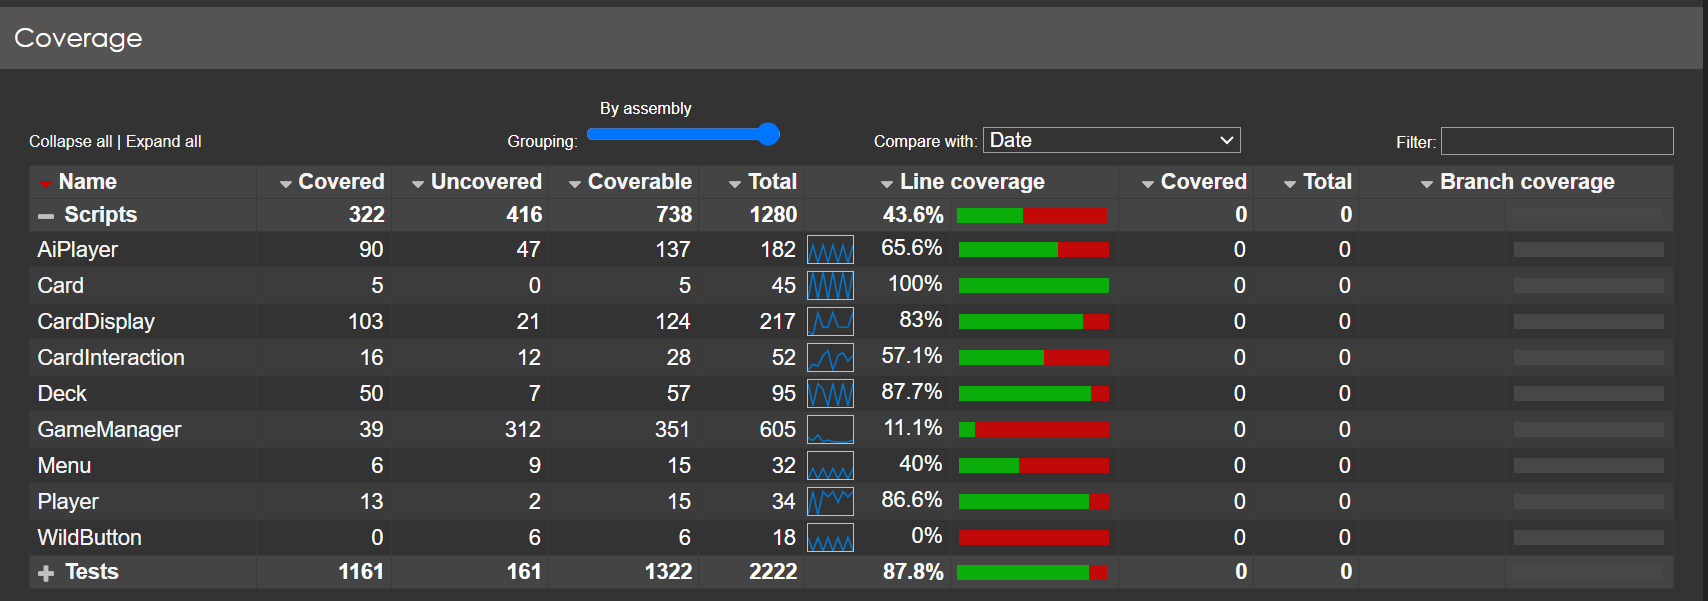
\includegraphics[width=1.1\textwidth]{coverage3.png}  % Change file name if needed
    \caption{Code Coverage Report}
    \label{fig:coverage}
\end{figure}

\newpage{}

\bibliographystyle{plainnat}
\bibliography{../../refs/References}


\section{Appendix --- Reflection}

\begin{enumerate}
  \item What went well while writing this deliverable? The writing process of functional requirement evaluation and nonfunctional requirements evaluation section went well because we had already performed all the tests before and the result is relatively straightforward. We also had a lot of references back to our VnV Plan document and checked if the test cases were still valid. If we think the test case is still eligible, we proceeded to test the planned test case. Sections 9 and 10 also went well since we directly referred back to our SRS document
  \item What pain points did you experience during this deliverable, and how did you resolve them?\\\\
  The units tests. When we were writing our code, we mostly tested everything manually and did not write unit tests. Therefore, we have to write formal unit tests for each of our scripts and perform the test and writing the result to our document. This took a lot of time, especially during midterm season. Next time, we will read the instructions carefully and ensure we do not miss any required elements.
  \item Which parts of this document stemmed from speaking to your client(s) or a proxy (e.g. your peers)?\\\\
  We communicate with other teams about what structure we should use for each section of this document since we are not quite sure about the structure required. After the communication, we followed the guideline of other teams, but modified some of them to better suit the nature of our project. Since one of our extras is the usability testing, we presented our software to several other friends and classmates so they can finish our survey. Most of them think we did pretty well on our game, but the quality of the user interface should be improved to maximize the user experience.
  \item In what ways was the Verification and Validation (VnV) Plan different from the activities that were actually conducted for VnV?\\\\
  The VnV plan only planning about what should we do for the testing of our software. Some of them are more abstract and may not be easily implements in the actual testing. Some of them may be meaningful when we make the plans, but could be useless when we actually perform the test. There are some requirements in our SRS document that are not covered in the VnV Plan, but we rediscover these when we actually perform the test. In general, the VnV plan is more abstract, and the content in VnV report in here is more substantial and better suited for the nature of our project.
\end{enumerate}

\end{document}
